\documentclass[a4paper, 11pt]{article}
\usepackage[cpp]{mypackage}
\usepackage{float}
\usepackage{amsmath}
\usepackage{graphicx}
\usepackage{geometry}
\usepackage{listings}
\geometry{scale=0.8}
% \linespread{1.5}
\usepackage[colorlinks,linkcolor=red]{hyperref}

\lstset{language=python}

\title{
\normalfont \normalsize
\textsc{School of Data and Computer Science, Sun Yat-sen University} \\ [25pt] %textsc small capital letters
\rule{\textwidth}{0.5pt} \\[0.4cm] % Thin top horizontal rule
\huge  Lab 4 Futoshiki Puzzle (Forward Checking)\\ % The assignment title
\rule{\textwidth}{2pt} \\[0.5cm] % Thick bottom horizontal rule
\author{17341015 Hongzheng Chen}
\date{\normalsize\today}
}

\begin{document}
\maketitle
\tableofcontents
\newpage

\section{Futoshiki}
Futoshiki is a board-based puzzle game, also known under the name Unequal. It is playable on a square board having a given fixed size ($4\times4$ for example).

The purpose of the game is to discover the digits hidden inside the board's cells; each cell is filled with a digit between 1 and the board's size. On each row and column each digit appears exactly once; therefore, when revealed, the digits of the board form a so-called Latin square.

At the beginning of the game some digits might be revealed. The board might also contain some inequalities between the board cells; these inequalities must be respected and can be used as clues in order to discover the remaining hidden digits.

Each puzzle is guaranteed to have a solution and only one.

You can play this game online: \url{http://www.futoshiki.org/}.
\begin{figure}[h]
  \centering
  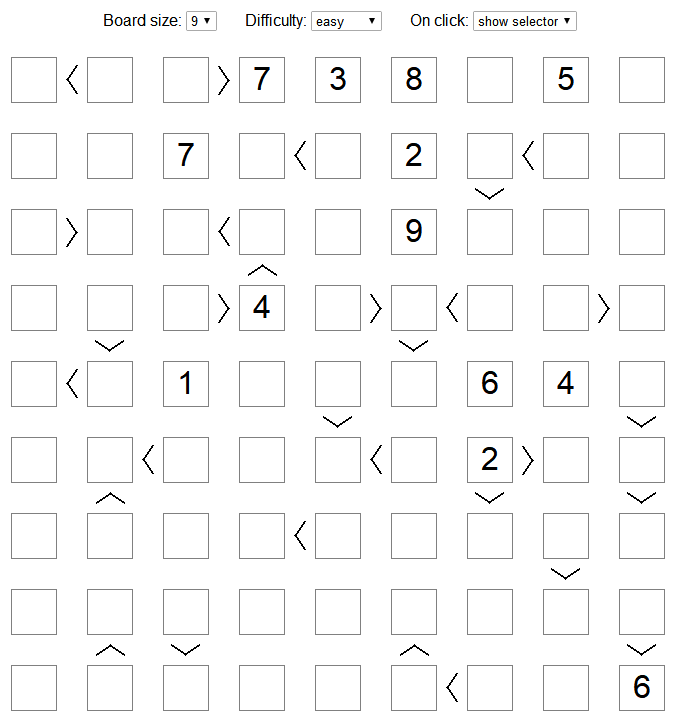
\includegraphics[width=7.5cm]{fig/futoshiki1}
  \qquad
  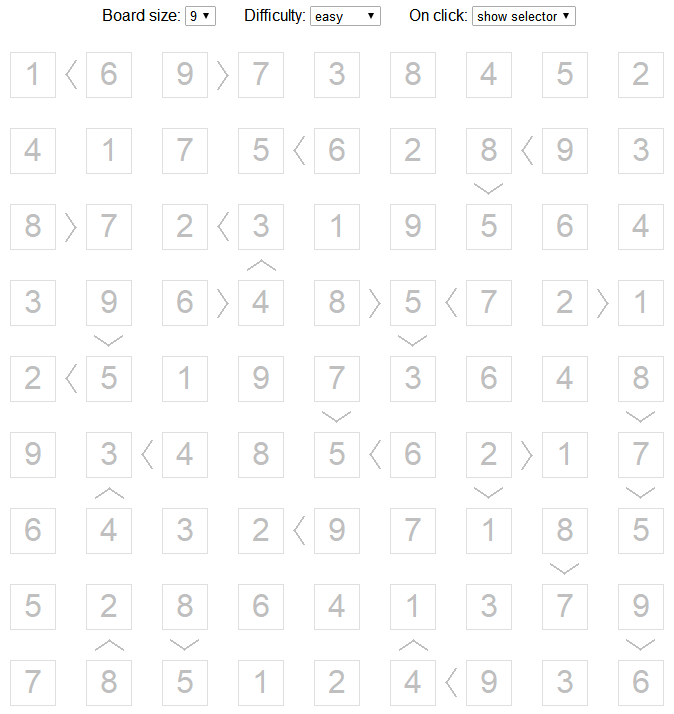
\includegraphics[width=7.5cm]{fig/futoshiki2}
  \label{fig:puzzle}
  \caption{An Futoshiki Puzzle}
\end{figure}

\section{Tasks}
\begin{enumerate}
\item Please solve the above Futoshiki puzzle ( Figure \ref{fig:puzzle} ) with forward checking algorithm.
\item Write the related codes and take a screenshot of the running results in the file named \textsf{E04\_YourNumber.pdf}, and send it to \textsf{ai\_201901@foxmail.com}.
\end{enumerate}

\section{Codes}
For better managing my game and the actions and making the separation of concerns (SoC), I encapsulate the state and actions in two classes.
One is \verb'Grid' that stores the value, valid numbers, and inequalities of a grid and also provide pruning functions.
The other is \verb'Futoshiki' which stores the whole chessboard and provides API for the searching algorithm to call.

I leverage a novel representation\footnote{It can also be found in the attachment \textsf{in.txt}.} to represent the states and the inequality constraints.
As shown below, the first $n$ lines gives the initial state where $0$ means grids that can be filled, otherwise, the grids are occupied at the first time.
Then the next several lines gives the inequalities, $(x,y)>(u,v)$ means the value of grid $(x,y)$ should be greater than the value of grid $(u,v)$.
In this representation, constraints checking becomes very easy and straightforward.
\begin{lstlisting}
0 0 0 0
0 0 0 0
0 0 0 0
0 0 0 3
(1,1) > (1,2)
(1,3) > (1,4)
(1,4) > (2,4)
(3,3) > (2,3)
\end{lstlisting}

Everytime setting a value, constraints propagation will be triggered.
The inequalities can be used to prune the domains of each grid by calling the \verb'prune_small_than' and \verb'prune_bigger_than' algorithm.
Notice though the initial state is at the very beginning of the input file, the values will be added to the class instance after the constraints are added first, since the known constraints can be used to prune the domains even when the searching has not begun.

All the codes are shown below and can also be found in \verb'futoshiki.py'.
\begin{lstlisting}
import sys, time
from copy import deepcopy

SIZE = int(sys.argv[1])

class Grid(object):
	def __init__(self,x,y,size):
		self.x = x
		self.y = y
		self.size = size
		self.value = -1
		self.valid = [i for i in range(1,size+1)]
		self.constraints = []

	def __str__(self):
		return str(self.value)

	def set_value(self,val):
		self.value = val
		# update current grid's domain
		self.valid = [val]

	def get_valid_num(self):
		return self.valid

	def get_valid_len(self):
		return len(self.valid)

	def add_constraint(self,c):
		self.constraints.append(c)

	def get_constraints(self):
		return self.constraints

	def del_num(self,num):
		if num == self.value:
			return
		try:
			index = self.valid.index(num)
			self.valid.pop(index)
		except:
			pass

	def prune_smaller_than(self,val):
		for i in range(val+1):
			self.del_num(i)

	def prune_bigger_than(self,val):
		for i in range(self.size,val-1,-1):
			self.del_num(i)

class Futoshiki(object):
	def __init__(self,size):
		self.size = size
		self.arr = []
		for i in range(size):
			self.arr.append([])
			for j in range(size):
				self.arr[i].append(Grid(i,j,size))

	def add(self,x,y,val):
		self.set_value(x,y,val)

	def add_constraint(self,grid1,op,grid2):
		grid1 = eval(grid1)
		grid2 = eval(grid2)
		x1, y1 = grid1[0]-1, grid1[1]-1
		x2, y2 = grid2[0]-1, grid2[1]-1
		self.arr[x1][y1].add_constraint((op,(x2,y2)))
		self.arr[x2][y2].add_constraint(('<' if op == '>' else '>',(x1,y1)))

	def ini_unassigned(self):
		self.unassigned = []
		for i in range(self.size):
			for j in range(self.size):
				if self.arr[i][j].value == -1:
					self.unassigned.append((i,j))

	def set_unassigned(self,x,y):
		self.unassigned.append((x,y))

	def get_unassigned(self): # at the same time pop out
		# Minimum Remaining Values Heuristics (MRV)
		self.unassigned.sort(key=lambda x: self.arr[x[0]][x[1]].get_valid_len())
		res = self.unassigned[0]
		self.unassigned = self.unassigned[1:]
		return self.arr[res[0]][res[1]]

	def get_unassigned_len(self):
		return len(self.unassigned)

	def get_valid_len(self,x,y):
		return self.arr[x][y].get_valid_len()

	def set_value(self,x,y,val):
		self.arr[x][y].set_value(val)
		# update row domain
		for j in range(self.size):
			if j != y:
				self.arr[x][j].del_num(val)
		# update column domain
		for i in range(self.size):
			if i != x:
				self.arr[i][y].del_num(val)
		# update constraints domain
		for c in self.arr[x][y].get_constraints():
			u, v = c[1][0], c[1][1]
			if c[0] == '<':
				self.arr[u][v].prune_smaller_than(val)
			elif c[0] == '>':
				self.arr[u][v].prune_bigger_than(val)

	def print(self):
		for i in range(self.size):
			print(*(self.arr[i]))
		print()

	def print_valid(self):
		for i in range(self.size):
			for j in range(self.size):
				print(self.arr[i][j].get_valid_num(),end=" ")
			print()
		print()

def FC(board,level):
	if board.get_unassigned_len() == 0:
		board.print()
		print("Time: {:.2f}s".format(time.time()-start))
		sys.exit()
	grid = board.get_unassigned()
	for d in grid.get_valid_num():
		# avoid restoring the pruned values
		currBoard = deepcopy(board)
		# while set, do constraints propagation
		currBoard.set_value(grid.x,grid.y,d)
		# FCCheck
		DWO = False
		for i in range(SIZE):
			for j in range(SIZE):
				if currBoard.get_valid_len(i,j) == 0:
					# print(i,j,currBoard.arr[i][j].get_valid_num())
					DWO = True
					break
		if not DWO:
			FC(currBoard,level+1)
	board.set_unassigned(grid.x,grid.y)

board = Futoshiki(SIZE)
toBeAdded = []
with open("in.txt","r") as file:
	for (i,line) in enumerate(file):
		if i < SIZE:
			lst = list(map(int,line.split()))
			for (j,val) in enumerate(lst):
				if val != 0:
					toBeAdded.append((i,j,val))
		else:
			grid1, op, grid2 = line.split()
			board.add_constraint(grid1,op,grid2)

# after all the constraints are read in
# add the known values (ensure pruning at first)
for (i,j,val) in toBeAdded:
	board.add(i,j,val)
board.ini_unassigned()

start = time.time()
FC(board,0)
\end{lstlisting}

\section{Results}
I firstly test my program on small cases as shown in Fig.~\ref{fig:res4}.
\begin{figure}[H]
\centering
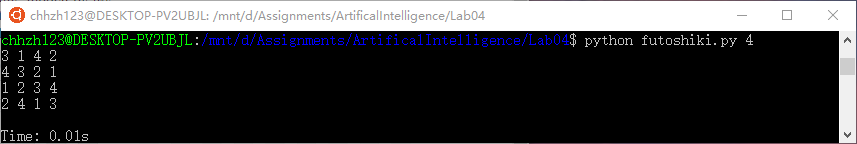
\includegraphics[width=\linewidth]{fig/result4.png}
\caption{Result of $4\times 4$ chessboard}
\label{fig:res4}
\end{figure}

And I search the solution of Fig.~\ref{fig:puzzle}, and the result is shown in Fig.~\ref{fig:res9}.
We can see that the result is correct and is the same as the provided answer.
\begin{figure}[H]
\centering
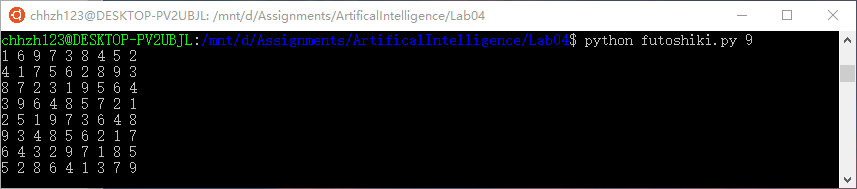
\includegraphics[width=\linewidth]{fig/result9.png}
\caption{Result of $9\times 9$ chessboard}
\label{fig:res9}
\end{figure}

%\clearpage
%\bibliography{E:/Papers/LiuLab}
%\bibliographystyle{apalike}
\end{document}